% Metodología del informe del proyecto final (modelo original BDL). Cifras del libro del proyecto y de
% ModeloOriginal/resultados; la tabla de hiperparámetros y la figura del pipeline las escribe generar.py.
\section{Metodología}\label{sec:metodologia}

Esta sección describe el problema, los datos y su análisis exploratorio, el pipeline, los modelos de referencia, el
modelo propuesto y el protocolo de evaluación; las cifras de desempeño se reservan para la sección~\ref{sec:resultados}.

\subsection{Formulación del problema y notación}\label{sec:formulacion}

Cada cliente $i$ se describe con un vector $\bm{x}_i \in \R^{p}$ ($p = 78$ columnas tras el preprocesamiento) y un
puntaje de propensión $s_i \in [0{,}114;\ 0{,}501]$, la columna \cp, que nunca vale 0 ni 1: es un puntaje, no un evento
observado. La tarea principal es la \textbf{regresión}: buscar $f: \R^p \to \R$ que minimice el error cuadrático medio,
\begin{equation}
  \mathcal{L}_R = \frac{1}{n}\sum_{i=1}^{n} (s_i - \hat{s}_i)^2, \qquad \rmse = \sqrt{\mathcal{L}_R},
  \label{eq:perdida}
\end{equation}
con el RMSE como métrica principal. La tarea secundaria es la \textbf{clasificación} del riesgo alto,
$y_i = \mathbf{1}[\,s_i > \tau\,]$, con $\tau$ el percentil 75 del puntaje estimado solo en el entrenamiento
($\tau = 0{,}3927$; $24{,}6$~\% de positivos), y el AUC como métrica. La Tabla~\ref{tab:notacion} resume la notación.

\begin{table}[htbp]
  \centering\small
  \caption{Notación principal.}
  \label{tab:notacion}
  \begin{tabular}{@{}>{\raggedright\arraybackslash}p{0.2\linewidth} >{\raggedright\arraybackslash}p{0.74\linewidth}@{}}
    \toprule
    Símbolo & Significado \\
    \midrule
    $\bm{x}_i \in \R^{p}$ & predictores del cliente $i$ tras el preprocesamiento ($p = 78$) \\
    $s_i$, $\hat{s}_i$ & puntaje \cp\ y su predicción \\
    $\tau$, $y_i$ & umbral de riesgo alto (percentil 75 del entrenamiento) y etiqueta $\mathbf{1}[s_i > \tau]$ \\
    $n$, $n_{\mathrm{te}}$ & clientes de entrenamiento ($38.978$) y de prueba ($9.745$) \\
    $F(\bm{x})$ & índice de BDL: una suma de árboles de regresión \\
    $z_i$, $K$ & clase latente del cliente (no se observa) y número de clases \\
    $\pi_k$, $c_k$, $\sigma$ & peso y desplazamiento de la clase $k$, y dispersión del error dentro de cada clase \\
    $\gamma_{ik}$ & probabilidad posterior de que el cliente $i$ pertenezca a la clase $k$ (paso E) \\
    $\tilde{s}_i$ & objetivo sin escalón: $s_i - \sum_k \gamma_{ik} c_k$ \\
    $\nu$, $d$, $M$, $\lambda$ & tasa de aprendizaje, profundidad de los árboles, intervalos por variable y penalización L2 de las hojas \\
    \bottomrule
  \end{tabular}
\end{table}

\subsection{Datos y análisis exploratorio}\label{sec:datos}

\paragraph{Fuente y tamaño.}
COFINFAD, \emph{Colombian Fintech Financial Analytics Dataset} \citep{munoz2025}, está publicado en Mendeley Data (DOI
10.17632/mhb4zn3258.1, licencia CC~BY~4.0). Describe a los clientes de una \emph{fintech} colombiana durante 2023 en dos
tablas: una con un registro por cliente ($48.723$ filas y $54$ columnas: perfil, tenencia de productos, uso digital,
satisfacción, resúmenes transaccionales y los objetivos) y otra con el detalle de $3.159.157$ transacciones. Los datos
son \textbf{sintéticos}: las conclusiones describen las reglas con que se generaron, no a clientes reales.

\paragraph{ETL.}
La auditoría del detalle no encontró montos no positivos, fechas nulas ni transacciones huérfanas, y eliminó $102$
transacciones duplicadas. Del detalle se derivaron doce variables de comportamiento por cliente (número de
transacciones; monto total, medio y mediano; recencia; días y meses activos; volatilidad del monto y proporción de cada
tipo de transacción), ninguna de las cuales usa el objetivo. Se eliminaron $17$ columnas con la evidencia de la
Tabla~\ref{tab:etl}. El único faltante que se conserva, \texttt{credit\_utilization\_ratio} ($37{,}4$~\% de los clientes
de entrenamiento), falta exactamente cuando el cliente no tiene tarjeta de crédito: es un \emph{no aplica} y se imputa
con cero. El conjunto final tiene $48$ predictores ($32$ numéricos, $9$ categóricos y $7$ booleanos), que el
preprocesamiento convierte en $p = 78$ columnas.

\begin{table}[tbp]
  \centering\small
  \caption{Columnas eliminadas en el ETL y razón de cada decisión (evidencia calculada solo con el entrenamiento).}
  \label{tab:etl}
  \begin{tabular}{@{}>{\raggedright\arraybackslash}p{0.34\linewidth} >{\raggedright\arraybackslash}p{0.6\linewidth}@{}}
    \toprule
    Columnas & Razón \\
    \midrule
    identificador del cliente & sin valor predictivo \\
    \ap & fuga de información: el puntaje se construyó a partir de ella (Figura~\ref{fig:objetivo}) \\
    valor del cliente y su segmento & son un segundo objetivo \\
    cuatro resúmenes transaccionales & duplican a otras columnas (dos con $r = 1{,}000$ con la frecuencia de transacciones) \\
    dos fechas & duplican a otras fechas \\
    tres fechas (\texttt{last\_survey\_date}, \texttt{first\_tx}, \texttt{last\_tx}) & sin señal ($\eta^2 = 0{,}0087$, $0{,}0046$ y $0{,}0044$) \\
    \texttt{nps\_score} & colineal con la satisfacción ($r = 0{,}917$) \\
    \texttt{occupation} & $35$ niveles sin señal ($\eta^2 = 0{,}0010$) \\
    dos columnas de texto & $50$~\% y $33$~\% de valores ausentes, sin mecanismo ni señal \\
    \bottomrule
  \end{tabular}
\end{table}

\paragraph{Hallazgos del análisis exploratorio.}
El puntaje tiene una distribución unimodal y asimétrica a la izquierda (asimetría $-0{,}61$; Figura~\ref{fig:objetivo},
izquierda), sin atípicos que tratar. Tres hallazgos condicionan el modelado. Primero, la edad solo toma seis valores
($29$, $30$, $44$, $45$, $59$ y $60$ años) agrupados en tres cohortes, en las que la proporción de riesgo alto va del
$8{,}7$ al $45{,}2$~\% sin crecer con la edad: una relación que un coeficiente lineal no representa y un árbol sí.
Segundo, \ap\ es la variable más asociada con el puntaje ($r = -0{,}876$; explica el $76{,}8$~\% de su varianza) y su
media desciende en escalones casi idénticos ($-0{,}0498$, $-0{,}0496$, $-0{,}0508$ y $-0{,}0496$; Figura~\ref{fig:objetivo},
derecha), con la misma dispersión ($0{,}032$) en cada nivel. Un paso constante es la firma de una regla de generación:
la variable se excluye por fuga de información \citep{kaufman2012}, y su escalón queda en el puntaje como un ruido de
cinco niveles que ningún predictor explica (al intentar predecirla con los demás, el AUC es $0{,}50$). Ese hallazgo
motiva el modelo propuesto. Tercero, sin ella la señal se concentra en pocas variables: correlaciones de Spearman de
$-0{,}279$ (frecuencia de uso de la aplicación), $+0{,}210$ (edad), $-0{,}190$ (satisfacción) y $-0{,}164$
(satisfacción de base), mientras que las doce variables transaccionales no aportan ($|\rho| \leq 0{,}018$).

\begin{figure}[tbp]
  \centering
  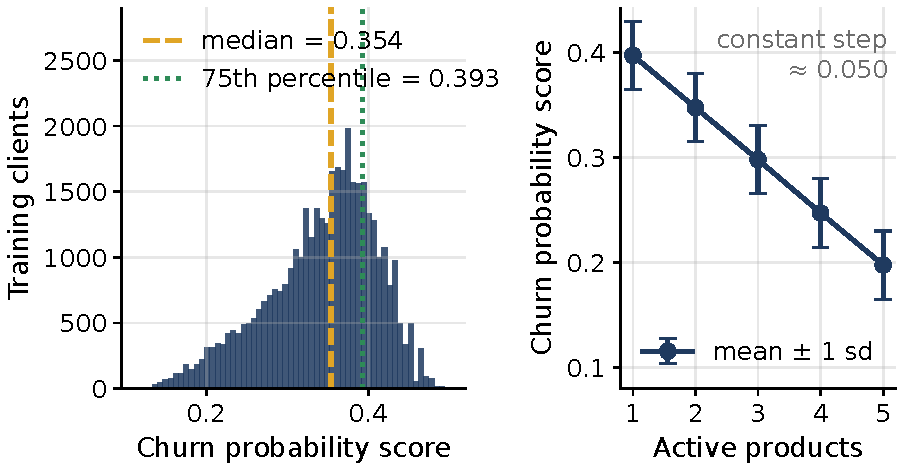
\includegraphics[width=\linewidth]{fig_target.pdf}
  \caption{Izquierda: distribución del puntaje \cp\ en el entrenamiento, con la mediana y el percentil 75 (umbral del
  riesgo alto). Derecha: media y desviación del puntaje por número de productos activos; el paso constante, de unos
  $0{,}050$, delata la regla con la que se generó el puntaje y justifica excluir esa variable.}
  \label{fig:objetivo}
\end{figure}

\subsection{Pipeline y control de fugas}\label{sec:pipeline}

La Figura~\ref{fig:pipeline} resume el pipeline. La partición va antes que todo lo demás: $80/20$ por índices con
semilla $42$ ($n = 38.978$ clientes de entrenamiento y $n_{\mathrm{te}} = 9.745$ de prueba), aleatoria y no por
posición porque el archivo está ordenado por cohortes. La evidencia para eliminar columnas, el umbral $\tau$ y la
fecha de corte de la recencia salen solo de los clientes de entrenamiento, y la prueba no se toca hasta la evaluación
final. El preprocesamiento (imputación, estandarización de las numéricas y booleanas y codificación de las categóricas
con indicadoras) vive dentro de la tubería de cada modelo, de modo que se ajusta solo con las filas de entrenamiento de
cada pliegue.

\begin{figure}[tbp]
  \centering
  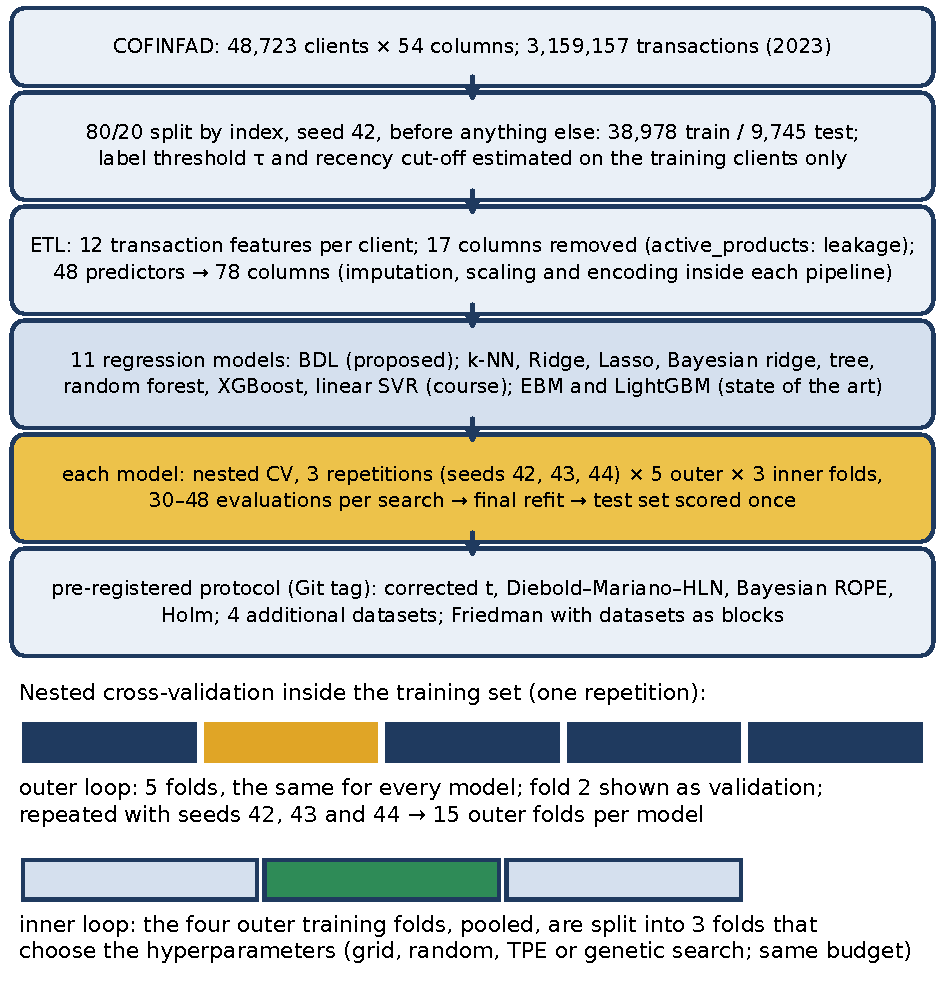
\includegraphics[width=\linewidth]{fig_pipeline.pdf}
  \caption{Pipeline del proyecto final y validación cruzada anidada de cada modelo. La partición se hace primero; el
  bucle externo produce la métrica que se reporta y el interno elige los hiperparámetros; el modelo final se reajusta
  con todo el entrenamiento y toca la prueba una sola vez.}
  \label{fig:pipeline}
\end{figure}

La recencia de un cliente es $\text{corte} - u$, con $u$ la fecha de su última transacción. Antes, la fecha de corte
se tomaba de todo el detalle, que incluye a los clientes de prueba; ahora sale solo del entrenamiento. La corrección
no cambia ningún dato (la fecha es la misma, el 29 de diciembre de 2023) y, además, no podía cambiar un resultado,
porque todos los modelos estandarizan la recencia con la media y la desviación del entrenamiento:
\begin{equation}
  z = \frac{(\text{corte} - u) - (\text{corte} - \bar u)}{s_u} = -\frac{u - \bar u}{s_u},
  \label{eq:recencia}
\end{equation}
que no contiene la fecha de corte. La auditoría de fugas \citep{kapoor2023} comprobó, además, que ningún cliente está
en las dos particiones, que el umbral se estima solo con el entrenamiento y que ningún modelo recibe \ap.

\subsection{Modelos de referencia}\label{sec:referencias}

El modelo propuesto se compara con todos los modelos de regresión del curso: $k$ vecinos más cercanos, Ridge, Lasso,
regresión bayesiana \citep{mackay1992}, árbol de decisión CART, Random Forest \citep{breiman2001}, XGBoost
\citep{chen2016xgboost} y SVR, en su versión lineal porque la de kernel RBF no escala a $38.978$ filas. Se añaden dos
métodos del estado del arte: la EBM \citep{nori2019interpretml} y LightGBM \citep{ke2017}. Todos usan las mismas
particiones, el mismo preprocesamiento y un presupuesto comparable: tantas evaluaciones de hiperparámetros como puntos
tiene la rejilla del modelo (de $30$ a $48$). Para cada benchmark se usa el mejor de cuatro optimizadores (rejilla,
búsqueda aleatoria, TPE de Optuna \citep{akiba2019} y un algoritmo genético), elegido en la entrega anterior; para BDL y
LightGBM, el protocolo fijó TPE. La regresión bayesiana no tiene búsqueda: estima las precisiones del ruido y de los
pesos por máxima evidencia en cada ajuste. La Tabla~\ref{tab:hiperparametros} da el espacio de búsqueda y los
hiperparámetros finales de cada modelo.

\begin{table}[tbp]
  \centering\scriptsize\setlength{\tabcolsep}{3pt}
  \caption{Espacios de búsqueda e hiperparámetros finales de cada modelo de regresión: optimizador elegido con su presupuesto (evaluaciones por búsqueda) y valores que fijó la búsqueda sobre todo el entrenamiento (repetición de la semilla 42).}
  \label{tab:hiperparametros}
  \begin{tabular}{>{\raggedright\arraybackslash}p{0.13\linewidth} >{\raggedright\arraybackslash}p{0.09\linewidth} >{\raggedright\arraybackslash}p{0.38\linewidth} >{\raggedright\arraybackslash}p{0.32\linewidth}}
    \toprule
    Modelo & Búsqueda & Espacio de búsqueda & Hiperparámetros finales \\
    \midrule
    BDL (propuesto) & TPE (30) & $\nu \in [0{,}05;\,1]$ (log); $d \in [1, 6]$; mín. por hoja $\in [5, 200]$ (log); $\lambda \in [0{,}01;\,10]$ (log); bins $M \in [32, 1024]$ (log); $K \in \{$BIC$, 1\}$ & $\nu$ = $0{,}5816$; $d$ = 1; mín. hoja = 88; $\lambda$ = $0{,}0151$; $M$ = 885; $K$ = BIC \\
    XGBoost & TPE (32) & árboles $\in [100, 1000]$ (log); profundidad $\in [2, 10]$; tasa $\in [10^{-3};\,0{,}3]$ (log); submuestreo de filas y de columnas $\in [0{,}5;\,1]$; $\lambda \in [0{,}01;\,10]$ (log); peso mín. por hoja $\in [1, 50]$ (log) & árboles = 512; prof. = 2; tasa = $0{,}0236$; filas = $0{,}80$; columnas = $0{,}73$; $\lambda$ = $0{,}216$; peso mín. = 31 \\
    LightGBM & TPE (32) & árboles $\in [100, 1000]$ (log); hojas $\in [4, 127]$ (log); tasa $\in [10^{-3};\,0{,}3]$ (log); submuestreo de filas y de columnas $\in [0{,}5;\,1]$; $\lambda \in [0{,}01;\,10]$ (log); mín. por hoja $\in [5, 200]$ (log) & árboles = 260; hojas = 4; tasa = $0{,}0508$; filas = $0{,}76$; columnas = $0{,}54$; $\lambda$ = $1{,}686$; mín. hoja = 104 \\
    EBM & rejilla (36) & tasa $\in [0{,}008;\,0{,}1]$ (log); hojas $\in \{2, 3, 4\}$; mín. por hoja $\in [2, 200]$ (log); interacciones $\in [0, 20]$; bins $\in [64, 1024]$ (log) & interacciones = 0; tasa = $8{,}0 \times 10^{-3}$; hojas = 3; mín. hoja = 20; bolsas = 8 \\
    Random Forest & rejilla (36) & profundidad $\in [4, 40]$; variables por corte $\in \{\sqrt{p}, \log_2 p, 0{,}3, 0{,}5\}$; mín. por hoja $\in [1, 100]$ (log); 100 árboles en la búsqueda y 300 en el final & prof. = 8; variables = $0{,}50$; mín. hoja = 50; árboles = 300 \\
    Árbol de decisión & genética (48) & profundidad $\in [3, 30]$; mín. por hoja $\in [1, 300]$ (log); poda $\alpha_{\mathrm{ccp}} \in [10^{-8}, 10^{-4}]$ (log) & prof. = 13; mín. hoja = 101; $\alpha_{\mathrm{ccp}}$ = $1{,}8 \times 10^{-6}$ \\
    Ridge & genética (30) & $\alpha \in [10^{-3}, 10^{5}]$ (log) & $\alpha$ = $613{,}9$ \\
    Lasso & genética (30) & $\alpha \in [10^{-6}, 10^{-1}]$ (log) & $\alpha$ = $1{,}1 \times 10^{-4}$ \\
    Regresión bayesiana & -- & sin búsqueda: las precisiones del ruido y de los pesos se estiman por máxima evidencia en cada ajuste & $\hat\alpha = 262{,}2$; $\hat\lambda = 76.586$ (precisiones estimadas) \\
    SVR lineal & TPE (30) & $C \in [10^{-3}, 10^{2}]$ (log); $\varepsilon \in [10^{-4};\,0{,}05]$ (log) & $C$ = $46{,}43$; $\varepsilon$ = $3{,}8 \times 10^{-4}$ \\
    k-NN & rejilla (32) & $k \in [5, 600]$ (entero, log); pesos uniformes o por distancia; métrica $L_q$, $q \in \{1, 2\}$ & $k$ = 80; $q$ = 1; pesos = distancia \\
    \bottomrule
  \end{tabular}
  \par\smallskip\begin{minipage}{0.97\linewidth}\scriptsize (log): búsqueda en escala logarítmica. El presupuesto es el número de puntos de la rejilla del modelo y se aplica igual con los cuatro optimizadores (rejilla, aleatoria, TPE y genética); el optimizador de cada benchmark es el mejor de los cuatro en el Entregable 3, y el de BDL y LightGBM quedó fijado en el protocolo. En BDL, $\nu$ es la tasa de aprendizaje, $d$ la profundidad de los árboles, $\lambda$ la penalización L2 de las hojas, $M$ el número máximo de intervalos por variable y $K$ el número de clases latentes (BIC: elegido por el criterio BIC; con $K=1$ no hay mezcla).\end{minipage}
\end{table}


\subsection{Modelo propuesto: \emph{boosting} con desplazamiento latente (BDL)}\label{sec:modelo}

\paragraph{Formulación.}
Para un cliente con predictores $\bm{x}$ y puntaje $s$, BDL supone
\begin{equation}
  s = F(\bm{x}) + c_{z} + e, \qquad z \in \{1, \dots, K\}, \quad P(z = k) = \pi_k, \quad e \sim \mathcal{N}(0, \sigma^2),
  \label{eq:modelo}
\end{equation}
con $z$ independiente de $\bm{x}$ y de $e$. $F(\bm{x}) = \beta_0 + \nu \sum_{t=1}^{T} h_t(\bm{x})$ es una suma de árboles
de regresión de profundidad $d$ sobre las variables discretizadas en a lo sumo $M$ intervalos; con $d = 1$ es un modelo
aditivo, con una curva por variable. $z$ es la clase latente, $c_k$ el desplazamiento de la clase $k$, $\pi_k$ su peso y
$\sigma$ la dispersión dentro de cada clase. Con $K = 1$, BDL es el \emph{boosting} de mínimos cuadrados de
\citet{friedman2001}. La log-verosimilitud de $n$ clientes es
\begin{equation}
  \ell(F, \theta) = \sum_{i=1}^{n} \log \sum_{k=1}^{K} \pi_k\, \varphi_\sigma\big(s_i - F(\bm{x}_i) - c_k\big),
  \qquad \theta = (\pi, c, \sigma),
  \label{eq:vero}
\end{equation}
con $\varphi_\sigma$ la densidad normal de media $0$ y desviación $\sigma$. Los supuestos son tres: el desplazamiento es
aditivo y no depende de $\bm{x}$, la clase es independiente de los predictores y la dispersión es la misma en todas las
clases. En COFINFAD se cumplen (sección~\ref{sec:datos}); cuando no, el BIC elige $K = 1$ y BDL se reduce a un
\emph{boosting} de mínimos cuadrados.

\paragraph{Regla de aprendizaje: EM generalizado con paso de \emph{boosting}.}
Maximizar \eqref{eq:vero} directamente es difícil por la suma dentro del logaritmo; el algoritmo EM \citep{dempster1977}
la sustituye por una cota que sí se puede maximizar. Sea $r_i = s_i - F(\bm{x}_i)$ el residuo. El \textbf{paso E}
calcula la probabilidad de que el cliente $i$ pertenezca a la clase $k$:
\begin{equation}
  \gamma_{ik} = \frac{\pi_k\, \varphi_\sigma(r_i - c_k)}{\sum_{l} \pi_l\, \varphi_\sigma(r_i - c_l)}.
  \label{eq:paso-e}
\end{equation}
La esperanza de la log-verosimilitud completa es
$Q(F, \theta) = \sum_i \sum_k \gamma_{ik} \big[\log \pi_k - \log \sigma - (s_i - c_k - F(\bm{x}_i))^2/(2\sigma^2)\big]$
más una constante. Como $\sum_k \gamma_{ik} = 1$, el término cuadrático se separa en
$(\tilde{s}_i - F(\bm{x}_i))^2$ más una varianza que no depende de $F$, con
\begin{equation}
  \tilde{s}_i = s_i - \sum_{k} \gamma_{ik}\, c_k,
  \label{eq:sin-escalon}
\end{equation}
el \textbf{objetivo sin escalón}: el puntaje menos el desplazamiento esperado de su clase. Maximizar $Q$ en $F$ es, por
tanto, minimizar $\sum_i (\tilde{s}_i - F(\bm{x}_i))^2$, y en lugar de resolverlo del todo se dan $B$ pasos de
\emph{boosting}: cada uno ajusta un árbol $h$ al residuo $\tilde{s}_i - F(\bm{x}_i)$ y actualiza $F \leftarrow F + \nu h$.
Cada nodo del árbol elige la variable y el corte que maximizan la ganancia
\begin{equation}
  \frac{G_L^2}{N_L + \lambda} + \frac{G_R^2}{N_R + \lambda} - \frac{G^2}{N + \lambda},
  \qquad v = \frac{G}{N + \lambda},
  \label{eq:ganancia}
\end{equation}
donde $G$ y $N$ son la suma de residuos y el número de filas del nodo, $L$ y $R$ sus hijos y $v$ el valor de una hoja.
El \textbf{paso M} actualiza la mezcla con el índice ya actualizado:
\begin{equation}
  \pi_k = \frac{1}{n}\sum_i \gamma_{ik}, \qquad
  c_k = \frac{\sum_i \gamma_{ik}\, r_i}{\sum_i \gamma_{ik}}, \qquad
  \sigma^2 = \frac{1}{n}\sum_i \sum_k \gamma_{ik}\, (r_i - c_k)^2.
  \label{eq:paso-m}
\end{equation}
El Algoritmo~\ref{alg:bdl} reúne los pasos. El número de clases se elige con el BIC \citep{schwarz1978} sobre el
residuo del calentamiento, con una regla de parsimonia: solo cuentan las clases separadas por al menos $4\sigma$ y con
al menos el $1$~\% de las filas.

\begin{algorithm}[tbp]
  \caption{Ajuste de BDL.}
  \label{alg:bdl}
  \small
  \begin{algorithmic}[1]
    \Require datos $(\bm{x}_i, s_i)_{i=1}^{n}$; tasa $\nu$; profundidad $d$; intervalos $M$; mínimo por hoja; $\lambda$;
             vueltas $V = 400$; árboles por vuelta $B = 5$; calentamiento $T_0 = 100$; $K_{\max} = 8$; paciencia $P = 20$
    \Ensure índice $F$, mezcla $(\pi, c, \sigma)$ y residuos de calibración
    \State Repartir las filas al azar: ajuste ($80$~\%), validación ($10$~\%) y calibración ($10$~\%)
    \State Discretizar cada variable en a lo sumo $M$ intervalos con las filas de ajuste
    \State \textbf{Calentamiento} ($K = 1$): $F \gets \bar{s}$; sumar hasta $T_0$ árboles ajustados a $s_i - F(\bm{x}_i)$, con parada temprana en validación
    \State \textbf{Mezcla inicial}: para $K = 1, \dots, K_{\max}$, $K$-medias exacto en una dimensión sobre los residuos y EM de la mezcla; elegir $K$ por BIC con la regla de parsimonia
    \For{$v = 1, \dots, V$}
      \State \textbf{Paso E}: $\gamma_{ik}$ con \eqref{eq:paso-e} y $\tilde{s}_i$ con \eqref{eq:sin-escalon}
      \State \textbf{Boosting}: $B$ veces, ajustar un árbol $h$ a $\tilde{s}_i - F(\bm{x}_i)$ con \eqref{eq:ganancia} y hacer $F \gets F + \nu h$
      \State \textbf{Paso M}: $\pi$, $c$ y $\sigma$ con \eqref{eq:paso-m}
      \If{el error dentro de clase en validación no mejora en $P$ vueltas} \textbf{parar} \EndIf
    \EndFor
    \State Conservar los árboles y la mezcla de la mejor vuelta y guardar los residuos de calibración
  \end{algorithmic}
\end{algorithm}

\paragraph{Regla de salida.}
En regresión, la predicción es la media del modelo, $\hat{s}(\bm{x}) = F(\bm{x}) + \sum_k \pi_k c_k$. Con los residuos de
calibración se construyen conjuntos de predicción conformes \citep{vovk2005} que usan la densidad de la mezcla como
medida de conformidad: con escalones, cada conjunto es una unión de intervalos cortos, uno por nivel. En clasificación,
la probabilidad de riesgo alto sale del propio modelo como una probabilidad de excedencia:
\begin{equation}
  P(s > \tau \mid \bm{x}) = \sum_{k=1}^{K} \pi_k\, \Phi\!\left(\frac{F(\bm{x}) + c_k - \tau}{\sigma_r}\right),
  \label{eq:excedencia}
\end{equation}
con $\sigma_r$ la dispersión robusta del error dentro de clase medida en validación.

\paragraph{Sustento teórico.}
\emph{La verosimilitud no decrece}: si $\nu \in (0, 2)$ y $\lambda \ge 0$, cada vuelta del Algoritmo~\ref{alg:bdl}
cumple $\ell(F', \theta') \ge \ell(F, \theta)$, y con $\sigma \ge \sigma_{\min} > 0$ la sucesión converge. La razón es
que, por la descomposición de EM, $\ell(F', \theta') - \ell(F, \theta) \ge Q(F', \theta') - Q(F, \theta)$, y ningún paso
baja $Q$: un árbol con hojas de valor $v_l = S_l/(n_l + \lambda)$ cambia la suma de cuadrados en a lo sumo
$-\nu(2 - \nu)\sum_l S_l^2/(n_l + \lambda) \le 0$, y \eqref{eq:paso-m} es el máximo de $Q$ en $\theta$. Además, si las
filas de calibración y un cliente nuevo son intercambiables, los conjuntos de predicción tienen cobertura de al menos
$1 - \alpha$ sin suponer que el modelo sea correcto \citep{vovk2005}. Cada propiedad tiene una prueba unitaria que la
verifica numéricamente.

\paragraph{Implementación.}
\begin{sloppypar}
BDL está programado desde cero con \texttt{numpy} y \texttt{scipy}, en el archivo \texttt{original\_\allowbreak model.py}
del repositorio: la discretización, los árboles por histogramas, el EM de la mezcla, el BIC y la salida conforme. De
scikit-learn solo usa las clases base que dan la interfaz de ajuste y predicción, y la validación de las entradas; una
prueba automática falla si el módulo importa cualquier otra cosa. Las $23$ pruebas unitarias corren en integración continua.
\end{sloppypar}

\subsection{Protocolo de evaluación}\label{sec:protocolo}

\paragraph{Validación.}
Cada modelo se evalúa con validación cruzada anidada \citep{cawley2010}: tres repeticiones (semillas $42$, $43$ y $44$)
de un bucle externo de cinco pliegues, los mismos para todos los modelos, que producen $15$ métricas por modelo; dentro
de cada pliegue externo, un bucle interno de tres pliegues elige los hiperparámetros. El modelo final se reajusta con
todo el entrenamiento y se evalúa una sola vez en la prueba, con un intervalo \emph{bootstrap} BCa \citep{efron1987}.
Las métricas son el RMSE (principal), el MAE, el MAPE y el $R^2$.

\paragraph{Protocolo registrado.}
Antes de los experimentos definitivos se congeló un protocolo con una etiqueta de Git. Sus hipótesis confirmatorias
son que el RMSE de BDL es menor que el del mejor benchmark (H1) y que su AUC es mayor (H2). Fija cuatro pruebas por
benchmark, con Holm \citep{holm1979}: Wilcoxon de rangos con signo y la $t$ corregida sobre los $15$ pliegues, y una
permutación pareada y un \emph{bootstrap} pareado BCa sobre la prueba. BDL se declara superior si su media es mejor
que la del mejor benchmark, al menos tres de las cuatro pruebas rechazan, el efecto no es despreciable ($|\delta| \ge
0{,}147$ o $|d| \ge 0{,}2$) y, en los conjuntos adicionales, es mejor en al menos dos de cuatro y no es
significativamente peor en ninguno.

\paragraph{Pruebas de la guía de resultados.}
Para cumplir la combinación mínima que pide la guía para regresión tabular se añadieron, después del protocolo, la
$t$ corregida de \citet{nadeau2003}, Diebold-Mariano con la corrección de Harvey-Leybourne-Newbold
\citep{diebold1995,harvey1997} y la $t$ correlacionada bayesiana con región de equivalencia práctica de $\pm 0{,}0005$ en
RMSE \citep{benavoli2017}, cada una con Holm sobre las diez referencias; tamaños de efecto ($d$ de Cohen y $A_{12}$);
el \emph{Model Confidence Set} al $90$~\% \citep{hansen2011mcs}, y Friedman con la corrección de Iman-Davenport y
Nemenyi \citep{demsar2006} con los cinco conjuntos de datos como bloques, no los pliegues de uno solo.

\paragraph{Conjuntos adicionales y techo.}
Cuatro conjuntos públicos con objetivo continuo, elegidos antes de conocer el desempeño de ningún modelo: dos con una
variable categórica que desplaza el objetivo retirada a propósito (Seguros médicos y Eficiencia energética), la
situación para la que se diseñó BDL, y dos sin modificar como control (Abulón y Vivienda de California). En cada uno
se usan cinco pliegues externos con la semilla $42$. Como el puntaje se generó a partir de \ap, se calcula además el
techo que deja su exclusión: el error del predictor óptimo que conoce la fórmula del puntaje salvo esa variable.

\paragraph{Ablación.}
La variante registrada retira la mezcla ($K = 1$) y conserva todo lo demás; se compara con las mismas pruebas. Como
análisis exploratorios, se fija $K$ entre $1$ y $8$, se repite la comparación con fracciones del entrenamiento y se
mide la sensibilidad a cada hiperparámetro, a la semilla y al ruido.

\paragraph{Disponibilidad.}
El código, los resultados, el libro del proyecto y el dashboard están en
\url{https://github.com/RubenEsg/Prediccion-de-fuga-de-clientes-en-fintech}, archivado en Zenodo
(\href{https://doi.org/10.5281/zenodo.24356311}{10.5281/zenodo.24356311}); \texttt{generar.py} reproduce cada tabla,
prueba y figura de este informe.
